\documentclass{beamer}
\usepackage[backend=biber, style=authoryear, sorting=ynt ]{biblatex}
\usepackage{algorithm}
\usepackage{quantikz}
\usepackage{graphicx}
\usepackage{amsmath}
\usepackage{tikz}

\newcommand{\ts}{\textsuperscript}

\title{Circle Detection}
\author{Manav Seksaria}
\institute{IIT Madras}
\date{\today}

\begin{document}

\frame{\titlepage}

% ===FRAME===
\begin{frame}\frametitle{The Problem}
We need to find the mean radius and mean distance between the circles below

\begin{figure}
    \centering
    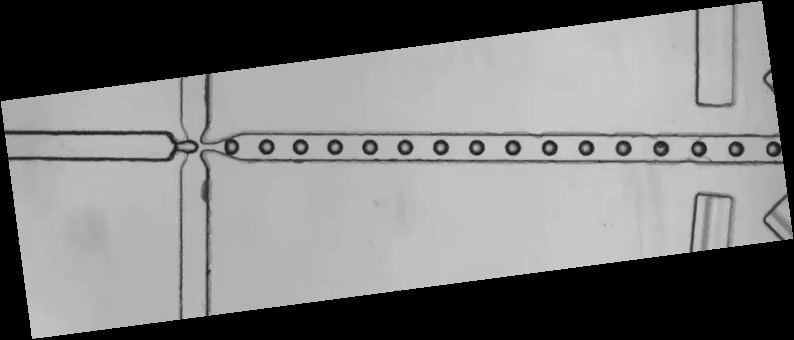
\includegraphics[width=\textwidth]{images_ppt/001.png}
    \caption{Array of circles}
\end{figure}
\end{frame}

% ===FRAME===
\begin{frame}\frametitle{\Huge How?}
{\huge Hough.}
\end{frame}

% ===FRAME===
\begin{frame}\frametitle{Steps}
We break our problem into the following step
\begin{itemize}
    \item Sobel Filter
    \item Coarse Hough Circle Transform (HCT)
    \item Find most likely radius $\pm \epsilon$
    \item Fine HCT with tuned params
    \item Find desired stats from obtained circles
\end{itemize}
\end{frame}

% ===FRAME===
\begin{frame}\frametitle{Hough Line Transform}

\begin{figure}
    \centering
    \includegraphics[width=\textwidth]{images_ppt/hough_line.png}
    \caption{Parametrised drawn through two points}
\end{figure}

Construct parametrised lines in Hesse normal form $r=x\cos \theta +y\sin \theta$ for all points
\end{frame}

% ===FRAME===
\begin{frame}\frametitle{Hough Line Transform}

Tabulate all values of $(r, \theta)$

\begin{table}[!ht]
    \centering
    \begin{tabular}{|l|l|l|l|l|l|}
    \hline
        $\theta$ & 15 & 30 & 45 & 60 & 75 \\ \hline
        $r_1$ (1\ts{st} Point) & 189 & 282 & 356 & 407 & 429 \\ \hline
        $r_2$ (2\ts{nd} Point) & 319 & 376 & 406 & 410 & 385 \\ \hline
    \end{tabular}
\end{table}

We can now see that $r_2 - r_1$ is minimum for $\theta=60 \implies$ line is most likely $408.5=x\cos 60 +y\sin 60$
\\
\\
A similar idea is extended to circles.
\end{frame}

% ===FRAME===
\begin{frame}\frametitle{Step 1: Sobel Filter}
%
\begin{figure}
    \centering
    \includegraphics[width=.5\textwidth]{images_ppt/img.png}
\end{figure}
%
\begin{align*}
\mathbf{G}_x =\begin{bmatrix}
+1&0&-1\\+2&0&-2\\+1&0&-1
\end{bmatrix}*\mathbf {A} ,\,
\mathbf{G}_y =\begin{bmatrix}
+1&+2&+1\\0&0&0\\-1&-2&-1
\end{bmatrix}*\mathbf {A}
\end{align*}
%
\begin{figure}
    \centering
    \includegraphics[width=.5\textwidth]{images_ppt/sobel.png}
\end{figure}
%
\end{frame}

% ===FRAME===
\begin{frame}\frametitle{Step 2: Coarse HCT}

Run with $R\in [1, 20]$ coarse sweep

\begin{figure}
    \centering
    \includegraphics[width=.75\textwidth]{images_ppt/chct.png}
\caption{Circles and some false positives}
\end{figure}

Find modal radius $R$, then allow for $\epsilon = 10\%$ error i.e new $R\in (R-\epsilon, R+\epsilon)$
\\
Here $R\in [6, 8]$

\end{frame}

% ===FRAME===
\begin{frame}\frametitle{Step 3: Fine HCT}

\begin{figure}
    \centering
    \includegraphics[width=.75\textwidth]{images_ppt/fhct.png}
    \caption{Circles and some false negatives}
\end{figure}

Again modal $R$ is taken, and all $(x,y)$ values are quantised to $(nR, mR)$ and modal $y$ is taken.
\\
Then at $R=7, y=147$
%
$$
X_i \in [266, 301, 336, 371, 406, 441, 476, 511, 546, 623, 665, 700, 735, 770]
$$
\end{frame}

% ===FRAME===
\begin{frame}\frametitle{\textit{Fin.}}
We can then find distance b/w circles via
$\frac{X_{i+1} - X_i}R - 2\, \forall\, X_i$

$$
\frac{X_{i+1} - X_i}R - 2 \in
[3, 3, 3, 3, 3, 3, 3, 3, 9, 4, 3, 3, 3]
$$

Therefore expected:
\begin{itemize}
    \item circle radius is $7$px
    \item inter-circular distance is $21$px ($3\times 7$px)
\end{itemize}
\end{frame}

\end{document}